\documentclass[addpoints]{exam}
  % Read in shared preamble for all homeworks
  %%%%%%%%%%%%%%%%%%%%%%%%%%%%%%%%%%%%%%%%%%%%%%%%%%%%%%%%%%%%%%%%%%%%
% This is the standard preamble for homework assignments and exams %
%                                                                  %
% -Joshua McNeill (joshua dot mcneill at uga dot edu)              %
%%%%%%%%%%%%%%%%%%%%%%%%%%%%%%%%%%%%%%%%%%%%%%%%%%%%%%%%%%%%%%%%%%%%
% Exam settings
\pointsinmargin
\pointformat{}

% Packages and settings
\usepackage{fontspec}
  \setmainfont{Charis SIL}
\usepackage{tikz}

%% Custom commands
% Instructions for a section
\newcommand{\instr}[1]{
  \begin{center}
    \fbox{
      \parbox{0.85\textwidth}
             {#1}
    }
  \end{center}
}
\newcommand{\lexi}[1]{\textit{#1}}
\newcommand{\gloss}[1]{`#1'}


  % Packages and settings
  \usepackage{graphicx}
    \graphicspath{{../figures/}}

  % Document information
  \title{Homework 1: Phonetics}
  \date{}

\begin{document}
  \maketitle

  % Header
  %%%%%%%%%%%%%%%%%%%%%%%%%%%%%%%%%%%%%%%%%%%%%%%%%%%%%%%%%%%%%%%%%%%%%%%
% This is the the header that all homework assignments and exams use. %
%                                                                     %
% -Joshua McNeill (joshua dot mcneill at uga dot edu)                 %
%%%%%%%%%%%%%%%%%%%%%%%%%%%%%%%%%%%%%%%%%%%%%%%%%%%%%%%%%%%%%%%%%%%%%%%
\noindent\makebox[0.5\textwidth][l]{Name:} \makebox[0.5\textwidth][r]{Course: LING2100, The Study of Language}\\
\makebox[0.5\textwidth][l]{Date:} \makebox[0.5\textwidth][r]{Instructor: Joshua McNeill}


  % Questions
    \instr{Give the IPA transcription of each word that you hear just as it's pronounced. Make sure to include stress. \emph{The audio can be found on eLC under assignments.} (1 point each)}

  \begin{questions}
      \parbox[t]{0.45\linewidth}{
        \question[1] \hrulefill
        \question[1] \hrulefill
        \question[1] \hrulefill
        \question[1] \hrulefill
        \question[1] \hrulefill
      }
      \hspace{0.1\linewidth}
      \parbox[t]{0.45\linewidth}{
        \question[1] \hrulefill
        \question[1] \hrulefill
        \question[1] \hrulefill
        \question[1] \hrulefill
        \question[1] \hrulefill
      }

    \instr{Give the IPA symbol for the \emph{consonant} that corresponds to the description. (1 point each)}
      \parbox[t]{0.45\linewidth}{
        \question[1] Voiced alveolar approximant: \hrulefill
        \question[1] Voiceless alveolar fricative: \hrulefill
        \question[1] Voiced dental fricative: \hrulefill
        \question[1] Voiceless labiodental fricative: \hrulefill
        \question[1] Voiceless velar stop: \hrulefill
        \question[1] Voiced labial-velar approximant: \hrulefill
      }
      \hspace{0.1\linewidth}
      \parbox[t]{0.45\linewidth}{
        \question[1] Voiced alveolar fricative: \hrulefill
        \question[1] Voiced alveolar nasal: \hrulefill
        \question[1] Voiced postalveolar fricative: \hrulefill
        \question[1] Voiced affricate: \hrulefill
        \question[1] Voiced palatal approximant: \hrulefill
        \question[1] Voiceless dental fricative: \hrulefill
      }

    \instr{Give the IPA symbol for the \emph{vowel} that corresponds to the description. (1 point each)}
      \parbox[t]{0.45\linewidth}{
        \question[1] High-mid back rounded: \hrulefill
        \question[1] Low-mid front unrounded: \hrulefill
        \question[1] High front unrounded: \hrulefill
      }
      \hspace{0.1\linewidth}
      \parbox[t]{0.45\linewidth}{
        \question[1] Near-low front unrounded: \hrulefill
        \question[1] Low-mid back rounded: \hrulefill
        \question[1] Near-high back rounded: \hrulefill
      }

    \instr{Give the description -- meaning the voicing, place of articulation, and manner of articulation -- that corresponds to the following \emph{consonant} IPA symbols. (1 point each)}
      \parbox[t]{0.45\linewidth}{
        \question[1] [d]: \hrulefill
        \question[1] [l]: \hrulefill
        \question[1] [h]: \hrulefill
        \question[1] [m]: \hrulefill
        \question[1] [ʃ]: \hrulefill
        \question[1] [t]: \hrulefill
      }
      \hspace{0.1\linewidth}
      \parbox[t]{0.45\linewidth}{
        \question[1] [g]: \hrulefill
        \question[1] [ʔ]: \hrulefill
        \question[1] [p]: \hrulefill
        \question[1] [tʃ]: \hrulefill
        \question[1] [ɾ]: \hrulefill
        \question[1] [b]: \hrulefill
      }

    \instr{Give the description -- meaning the height, advancement, and lip rounding -- that corresponds to the following \emph{vowel} IPA symbols. (1 point each)}
      \parbox[t]{0.45\linewidth}{
        \question[1] [u]: \hrulefill
        \question[1] [a]: \hrulefill
        \question[1] [ɑ]: \hrulefill
      }
      \hspace{0.1\linewidth}
      \parbox[t]{0.45\linewidth}{
        \question[1] [ɪ]: \hrulefill
        \question[1] [ʌ]: \hrulefill
        \question[1] [e]: \hrulefill
      }

    \instr{Give the word, in standard English spelling, that corresponds to the IPA transcription. (1 point each)}
      \parbox[t]{0.45\linewidth}{
        \question[1] [ˈfaɪ.næn.sɪŋ]: \hrulefill
        \question[1] [ɹəˈtɹækt]: \hrulefill
        \question[1] [ˈɹeɪl.ɹoʊd]: \hrulefill
        \question[1] [ˈæ.dʒɪ.teɪt]: \hrulefill
        \question[1] [ˈtɔl]: \hrulefill
        \question[1] [kæ.lɪˈbɹeɪ.ʃn̩]: \hrulefill
        \question[1] [ˈʃaʊ.təd]: \hrulefill
        \question[1] [ˈdʒæm]: \hrulefill
        \question[1] [əˈmæs]: \hrulefill
        \question[1] [bɑmˈbɑɹ.dəd]: \hrulefill
      }
      \hspace{0.1\linewidth}
      \parbox[t]{0.45\linewidth}{
        \question[1] [gəˈzɛl]: \hrulefill
        \question[1] [ˈdʒæz.mɪn]: \hrulefill
        \question[1] [ˈɔ.di.əns]: \hrulefill
        \question[1] [ˈmeɪ.ɹ̩]: \hrulefill
        \question[1] [dəˈɹɛk.tɪv]: \hrulefill
        \question[1] [ˈpɹoʊ.faɪl]: \hrulefill
        \question[1] [ˈwɹ̩st]: \hrulefill
        \question[1] [ˈtʃɑ.pi]: \hrulefill
        \question[1] [əˈpɹeɪ.zɹ̩]: \hrulefill
        \question[1] [ʌnˈhɪn.dɹ̩d]: \hrulefill
      }

    \instr{Give the syllable structure, as a tree diagram, for the following one syllable words. (1 point per label)}
      \question[1] [ˈðɛɹ]
      \vspace{\stretch{1}}
      \question[1] [ˈwaɪld]
      \vspace{\stretch{1}}
      \question[1] [ˈkæt]
      \vspace{\stretch{1}}
      \newpage
      \question[1] [ˈbɑɹk]
      \vspace{\stretch{1}}
      \question[1] [ˈkloʊz]
      \vspace{\stretch{1}}
      \question[1] [ˈnæt]
      \vspace{\stretch{1}}

    \instr{The two spectrograms below represent two different vowels. As best as you can, identify the approximate frequency of F1 and F2 for each. Be aware that three formants are visible. (1 point each)}
      \question[1]
        \begin{minipage}{0.45\linewidth}
          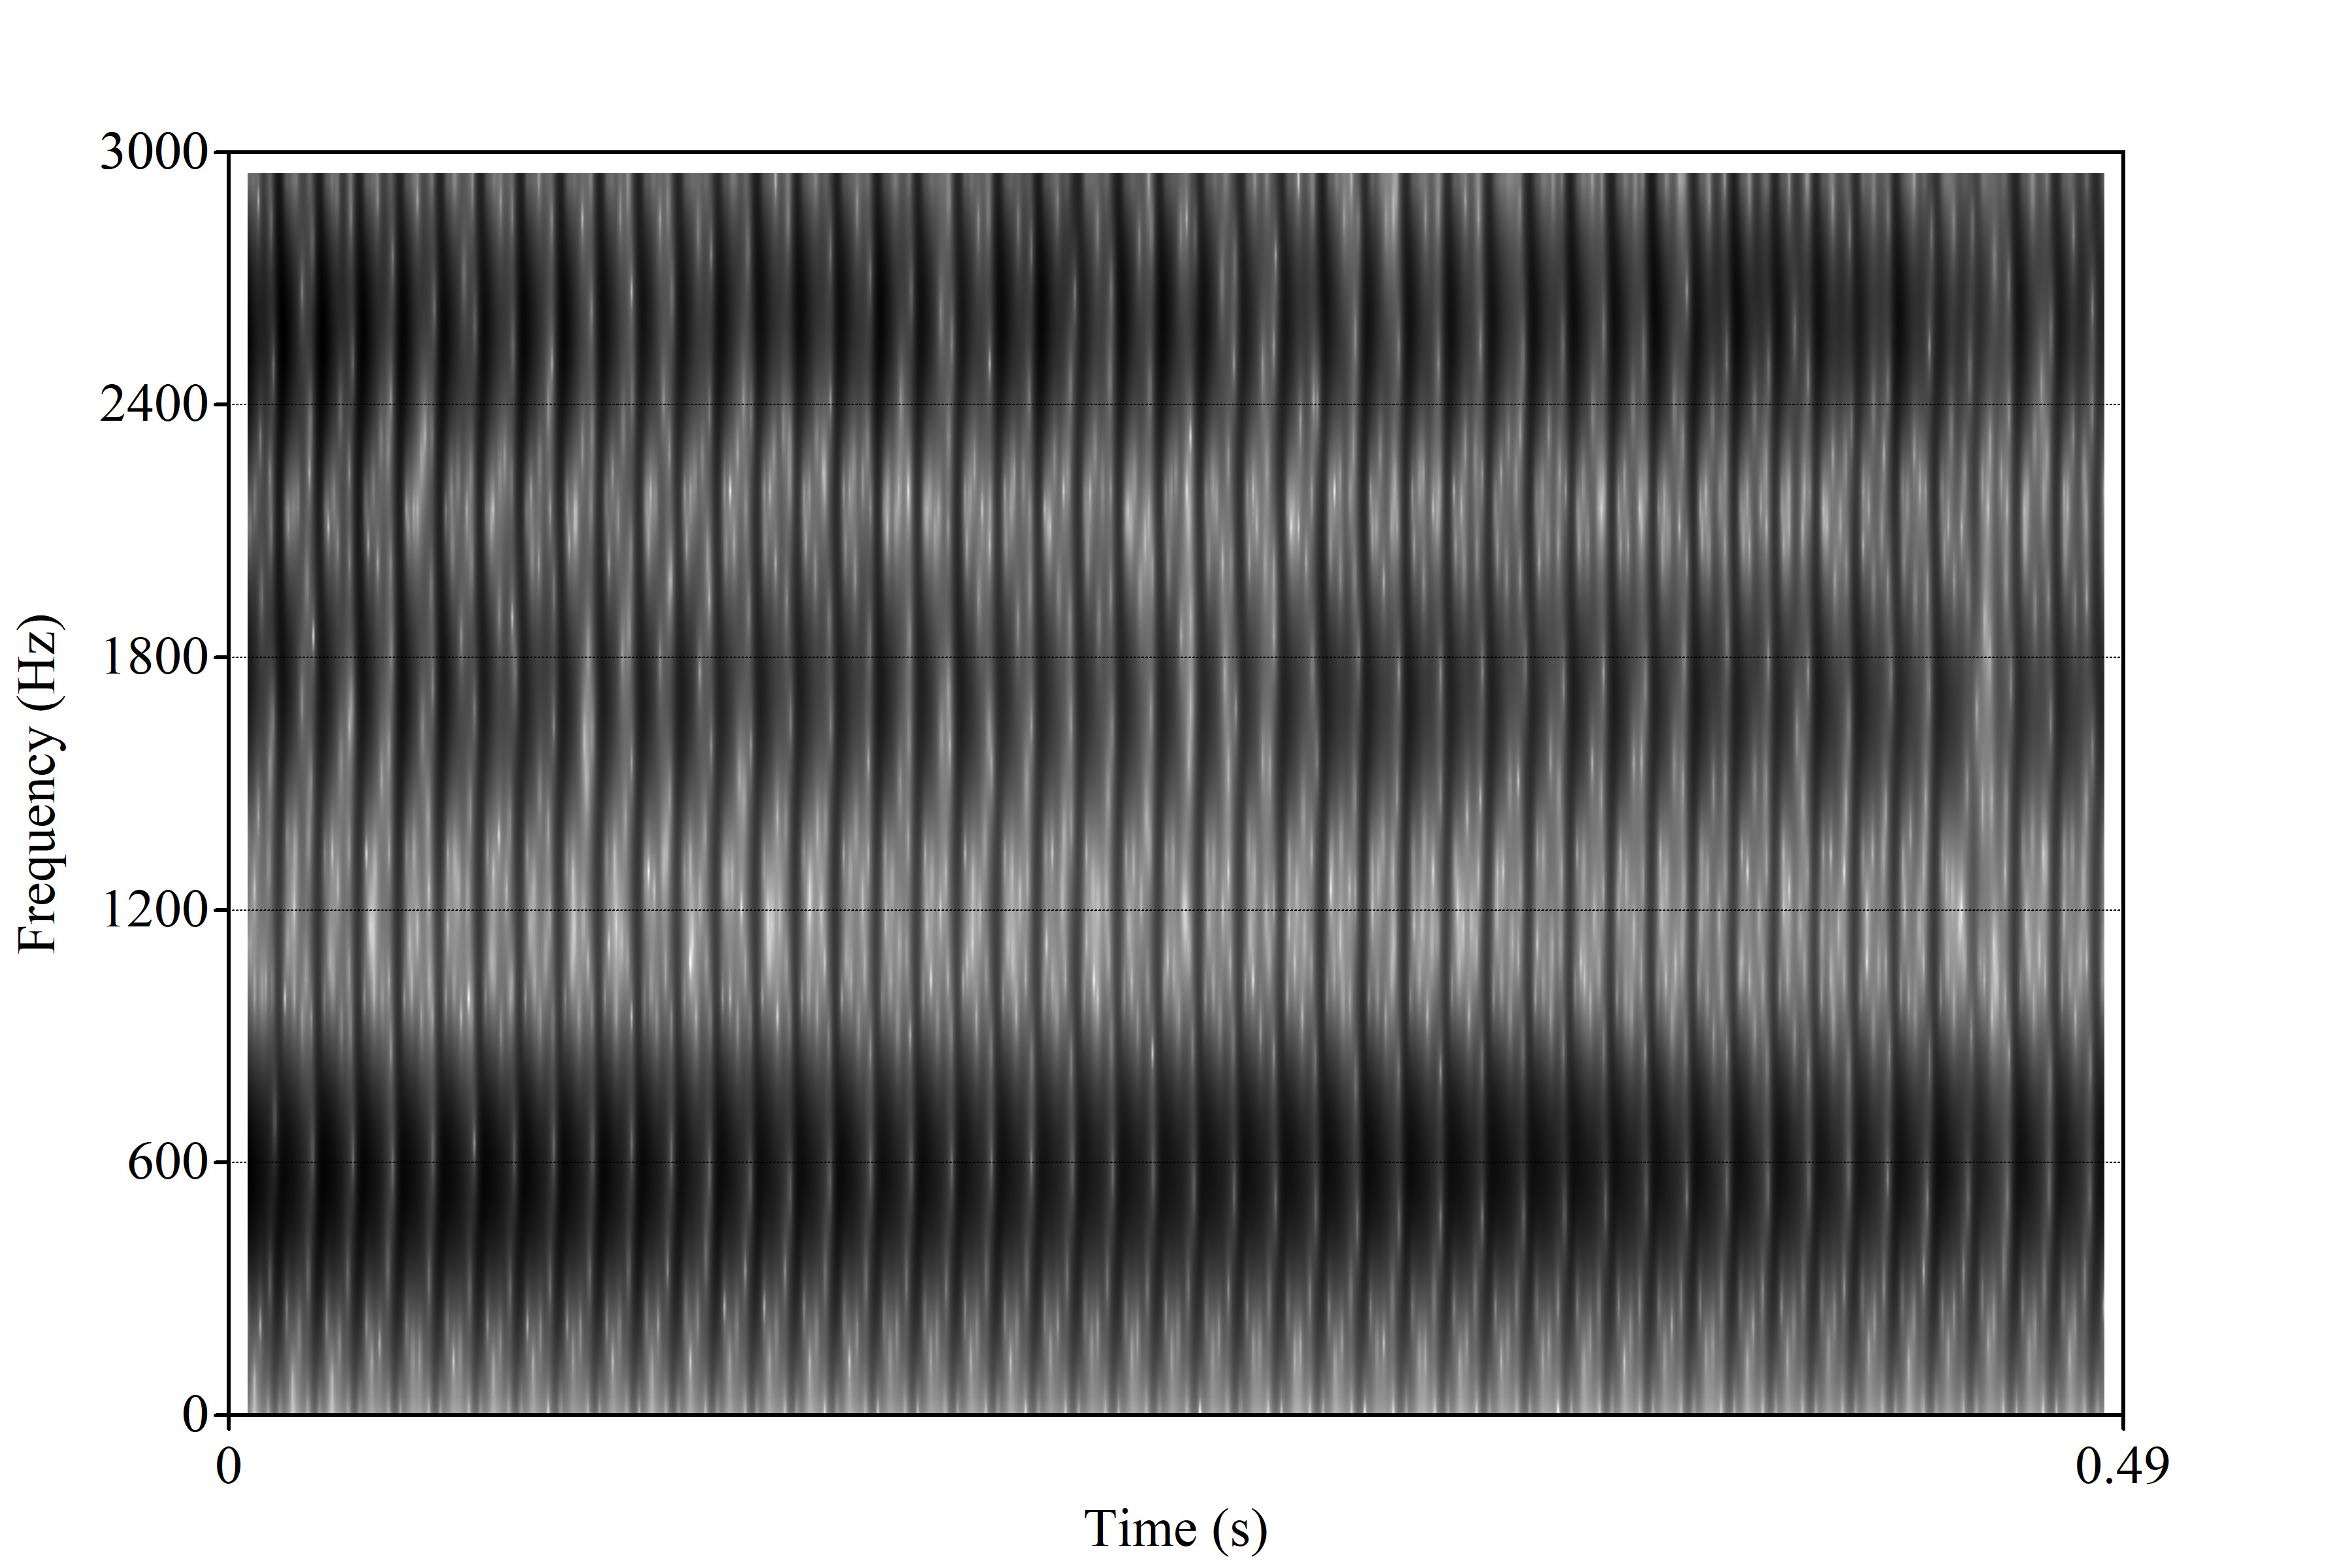
\includegraphics[scale=0.6]{vowel4.jpg}
        \end{minipage}\hspace{0.1\linewidth}
        \begin{minipage}{0.45\linewidth}
          \begin{itemize}
            \item[F1:] \hrulefill
            \item[F2:] \hrulefill
          \end{itemize}
        \end{minipage}
      \question[1]
        \begin{minipage}{0.45\linewidth}
          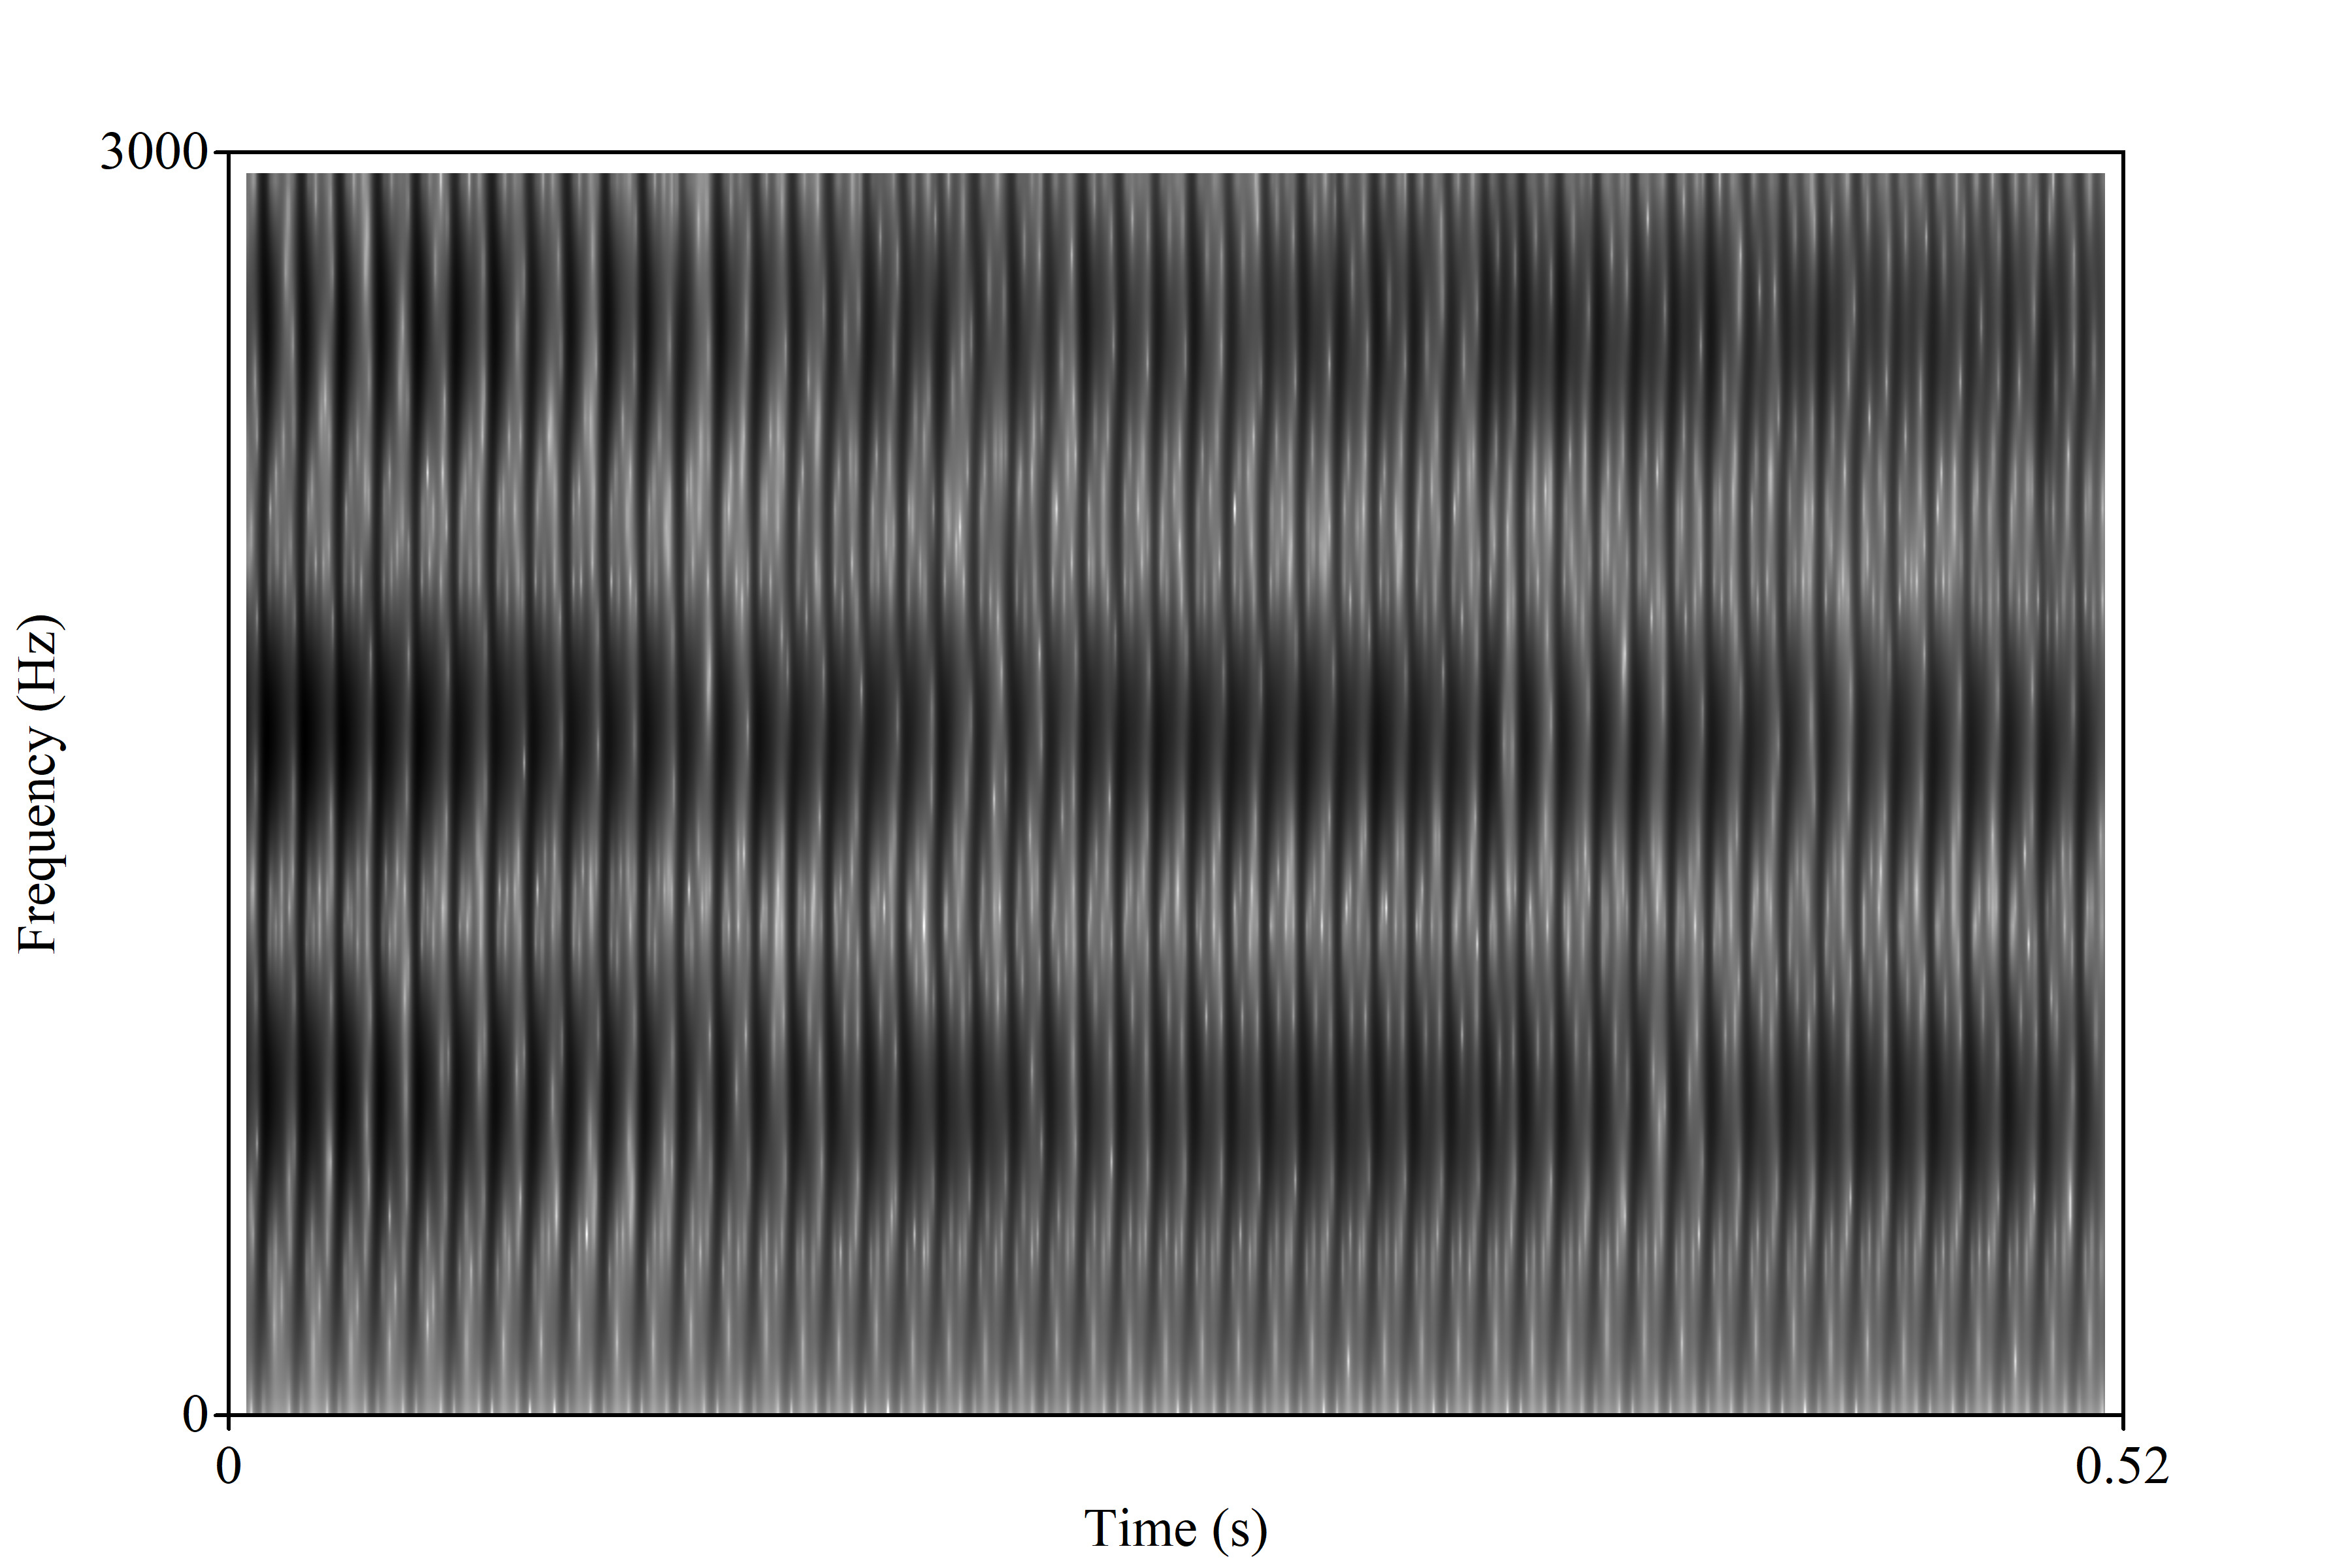
\includegraphics[scale=0.6]{vowel5.jpg}
        \end{minipage}\hspace{0.1\linewidth}
        \begin{minipage}{0.45\linewidth}
          \begin{itemize}
            \item[F1:] \hrulefill
            \item[F2:] \hrulefill
          \end{itemize}
        \end{minipage}
      \question[1]
        \begin{minipage}{0.45\linewidth}
          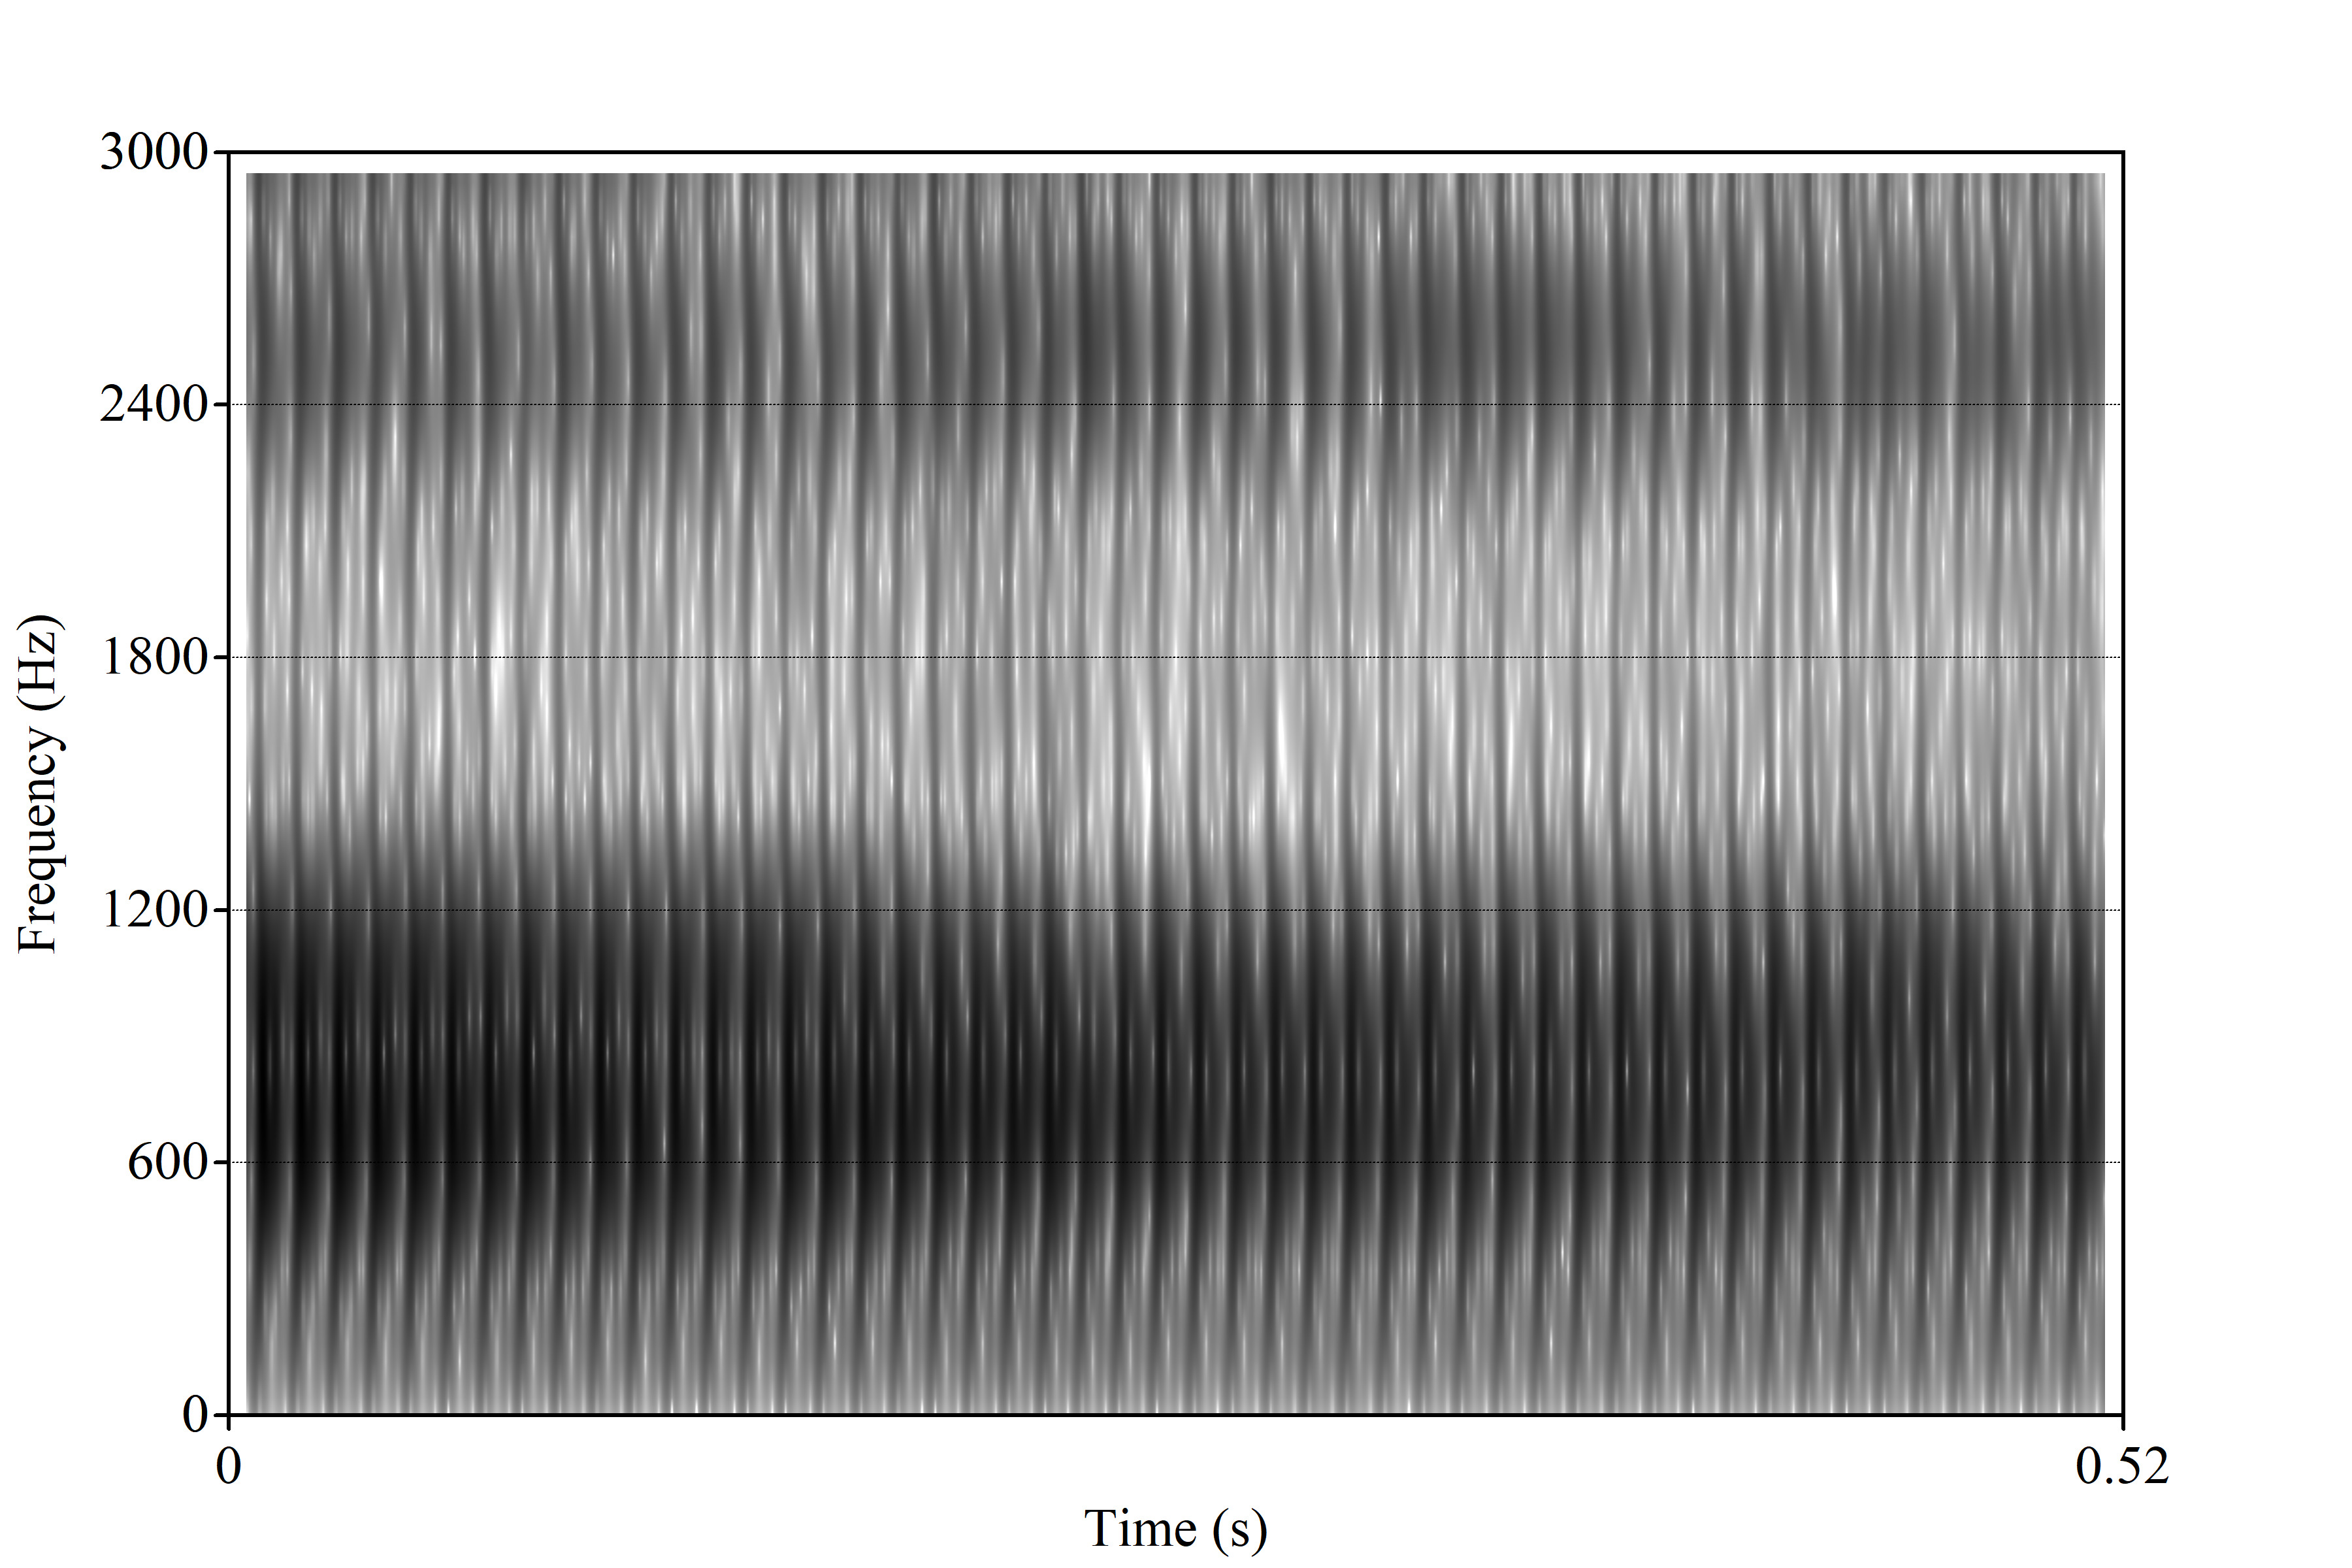
\includegraphics[scale=0.6]{vowel6.jpg}
        \end{minipage}\hspace{0.1\linewidth}
        \begin{minipage}{0.45\linewidth}
          \begin{itemize}
            \item[F1:] \hrulefill
            \item[F2:] \hrulefill
          \end{itemize}
        \end{minipage}
  \end{questions}

  \vspace{1.25cm}

  % Grade
  \begin{center}
    \gradetable[v][pages]
  \end{center}
\end{document}
